\section{Classification}

% - DATASET
%      - diverso rispetto a cluster
%      - features choice:
%          - soltanto numeriche
%          - tolto missing value
%          - tolto correlate con label
% - LABELIZZAZIONE
%     - mediana, media, pareto con percentuali e numero record
% - CLASSIFICAZIONE
%     - introduzione
%         - classificazione su pareto e su pareto con SMOTE
%         - grid search
%          - minmax scaler solo su alcuni
%         - cross validation con k-fold=5, split train-test 0.3
%     - MODELS
%         - DECISION TREE
%             - facile da interpretare
%         - RULE BASED
%             - facile da interpretare
%         - KNN
%             - sqrt(len(train))
%         - RANDOM FOREST
%             - facile?
%             - euristica con log/sqrt(len(features)), però in realtà max
%         - ADABOOST
%         - NAIVE
%             - assume feature condizionalmente indipendenti
%         - SVM
%         - NN
%     - PARLARE DELLA VALIDAZIONE PER OGNI MODELLO con OSSERVAZIONI SU
%         - grid search parametri ottimali
%         - validation metrics accuracy, f1, precision, recall
%         - validation curve (parlare di over/under fitting)
%         - learning curve
% - COMPARISON
%     - tra modelli con validation
%     - tra modelli con test
%     - tra modelli con ROC su TEST
%     - miglior modello con k-means?\\\\


The objective of the classification task was to identify strong players and weak players. In order to do that, the starting dataset used is the Players Dataset already defined. The goal here was to have more data. Hence, to consider more players, we set a lower threshold on the number of matches played (increasing the entries from 2997 to 3798).

\subsection{Pre-processing}

\paragraph{Label extraction}
The dataset is not provided with a label for this kind of classification task, so a homemade one was created taking into account the \verb|mean_rank_points| feature. First of all, it is necessary to discriminate between strong and weak players. To do this, there are several options, we have opted for:

\begin{itemize}
    \item \textbf{median}, this ensures to obtain balanced classes, hence $1899$ for each class
    \item \textbf{mean}, with the drawback of obtaining unbalanced classes: $3009$ weak, $789$ strong. This reminds us of the pattern identifies during clustering analysis, where 80\% of the players are weak and 20\% are strong. Of course, this better captures the inherent competitiveness of the game of tennis.
\end{itemize}

\begin{figure}[h]
	\centering
	\begin{minipage}{.5\textwidth}
		\centering
		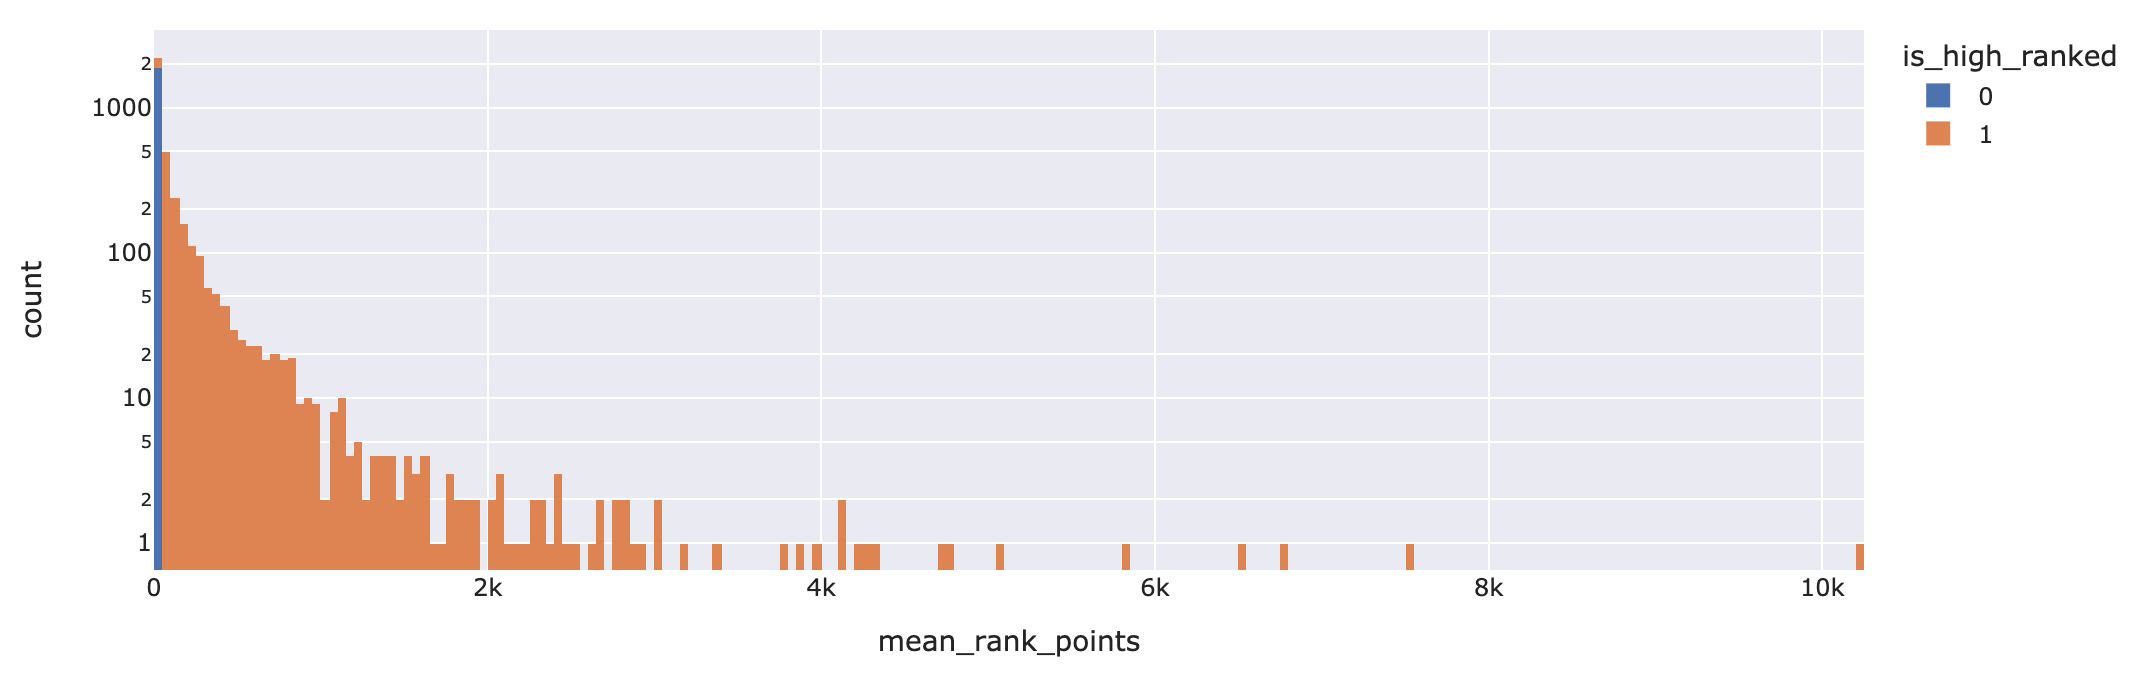
\includegraphics[width=\textwidth]{plots/median_splitting.png}
		\subcaption{Median}
		\label{fig:median_splitting}
	\end{minipage}%
	\begin{minipage}{.5\textwidth}
		\centering
		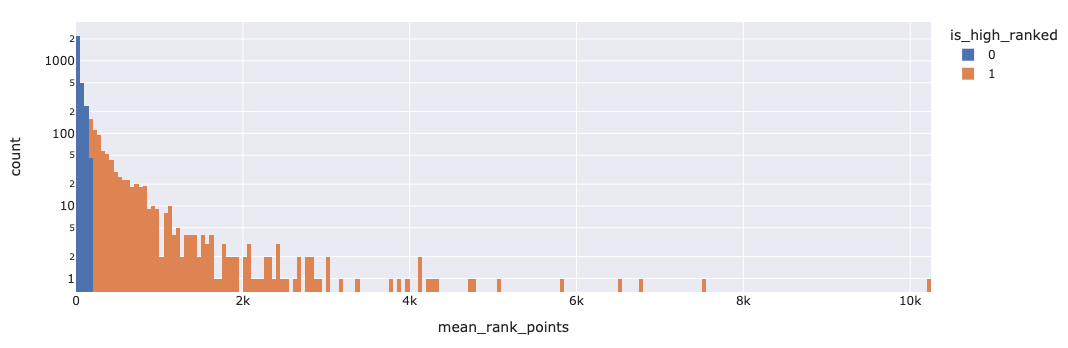
\includegraphics[width=\textwidth]{plots/mean_splitting.png}
		\subcaption{Mean}
		\label{fig:mean_splitting}
	\end{minipage}
	\captionof{figure}{Different options to split (\texit{log scale on y}).}
\end{figure}

\paragraph{Feature selection}
The next issue to address are the features to use for the classification purpose. We have only considered the numerical features, thus losing the information about the gender and the hand of the player. Then we dropped those features with a big amount of missing values such as the in-match statistics with the aim of maximizing the number of players in the dataset. Lastly, we dropped the derived features from rank points, such as \textit{max\_rank\_points}, \textit{last\_rank\_points}, \textit{variance\_rank\_points}. And of course in the end, \textit{mean\_rank\_points} was also deleted.

\paragraph{Normalization}
For all the algorithms, we applied a MinMaxScaler but the decision tree to make the interpretation more meaningful.

\paragraph{Oversampling}
In the case of the label extraction with the mean, the classes are unbalanced, so we thought of doing an experiment on the normal dataset and one on the dataset where SMOTE was applied on the minority class, which is an oversampling technique that synthesizes new records.


\subsection{Training and validation results}
% TODO CONFRONTO TRA LEARNING CURVE
Once the dataset was ready, we performed the analysis using different classifiers on both the median and mean computed label. But we decided to discuss the results obtained for the mean label, because we think that it better suits the definition of player's strength given the fact that it follows a Pareto distribution.
We tested different classification models and performed a grid search with a k-fold of 5 to find the best parameters. In the following part we will discuss the results on the dataset where SMOTE has been applied.

\paragraph{Results Analysis}
Regardless of the dataset used, we have noticed that the algorithms that perform well with some consistencies are the \textbf{Neural Network}, \textbf{Random Forest} and \textbf{SVM}. While those that get bad results with some consistencies are \textbf{Rule Based} and \textbf{Naive Bayes} (see Table \ref{tab:metrics-validation}).
The \textbf{Random Forests} have great results, and this is also due to the fact that data are tabular.
For \textbf{Naive Bayes}, this is probably due to the fact that the algorithm assumes the variables to be conditionally independent among each other.
About the \textbf{Neural Networks}, we chose to use very simple architectures; the one with the best performance has a hidden layer with 20 neurons and \verb|max_iter|=200. We also observed that for \verb|max_iter| values grater than 200, an overfitting behaviour occurs (Fig. \ref{fig:nn_validation_curve}).
We have also noticed that some of the optimal parameters that have been identified by the grid search do not match the heuristics. For \textbf{KNN} \verb|n_neighbors|, we have the best values of neighbor as 7 or 1 instead of $\sqrt{|training\ set|}$ (about 46) which is the value that can be proposed as heuristic. For \textbf{Random Forests}, we have optimal values with \verb|max_features|='None', instead of $\sqrt{\#\ avaiable\ attributes}$ or \textit{log\textsubscript{2}(\#\ available\ attributes)+1}.

\begin{figure}[h]
	\centering
	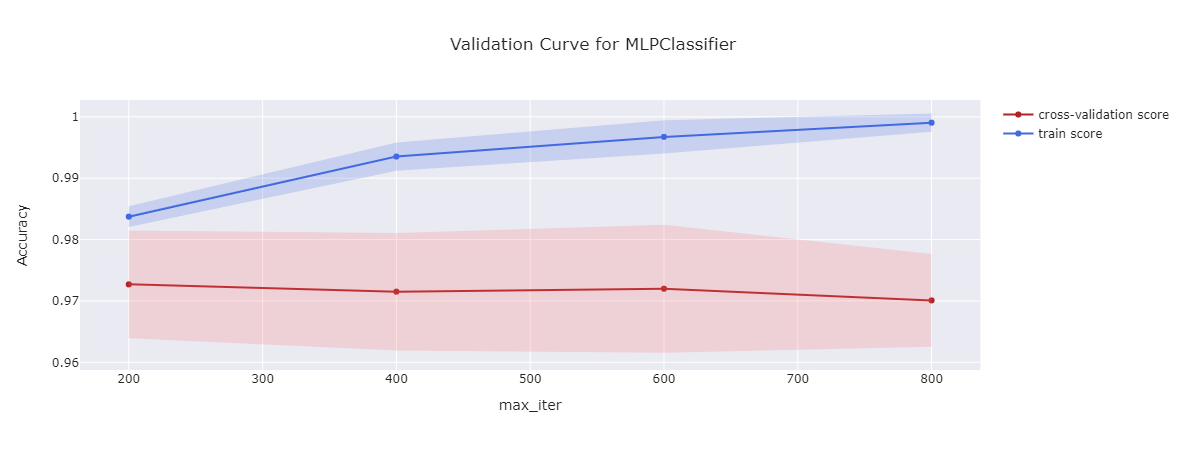
\includegraphics[width=\textwidth]{plots/classification/nn_validation_curve.png}
	\captionof{figure}{Neural Networks validation curve}
	\label{fig:nn_validation_curve}
\end{figure}

\paragraph{Would adding more data for the train have been useful?}
For each individual algorithm, we have defined a learning curve, which allows us to analyse the accuracy on the train set and on the validation set as the size of the dataset varies. What we can see in general, looking at the learning curves in figure X, is that the accuracy on the validation set initially has a very high standard deviation, but with more than 1800 samples it starts to converge. So we can say that most of the models would not have benefited much with the addition of new data. This means that probably, even using the starting dataset with a larger threshold of matches played, we would have obtained good results.
\begin{figure}[h]
\end{figure}


\begin{figure}[h]
	\centering
	\begin{minipage}{.48\textwidth}
	    \centering
    	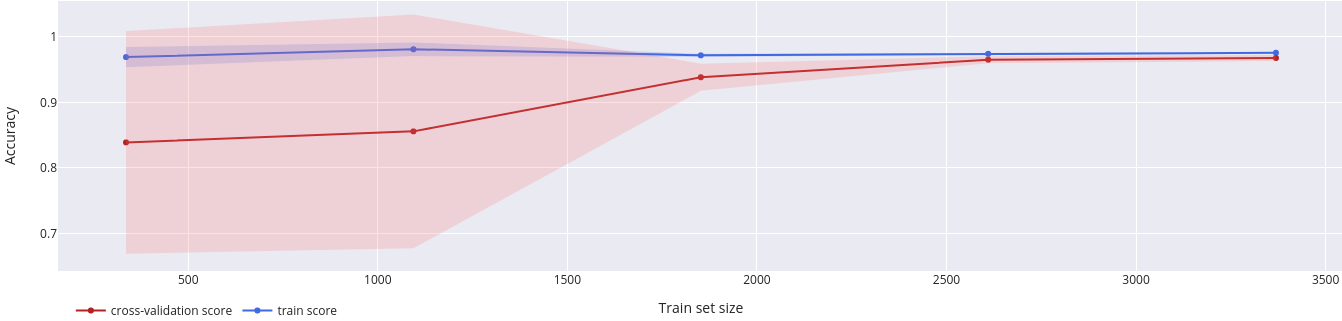
\includegraphics[width=\textwidth]{plots/classification/random_forest_learning_curve.png}
    	\label{fig:random_forest_learning_curve}
    	\subcaption{Random Forest}
	\end{minipage}
	\begin{minipage}{.48\textwidth}
	    \centering
		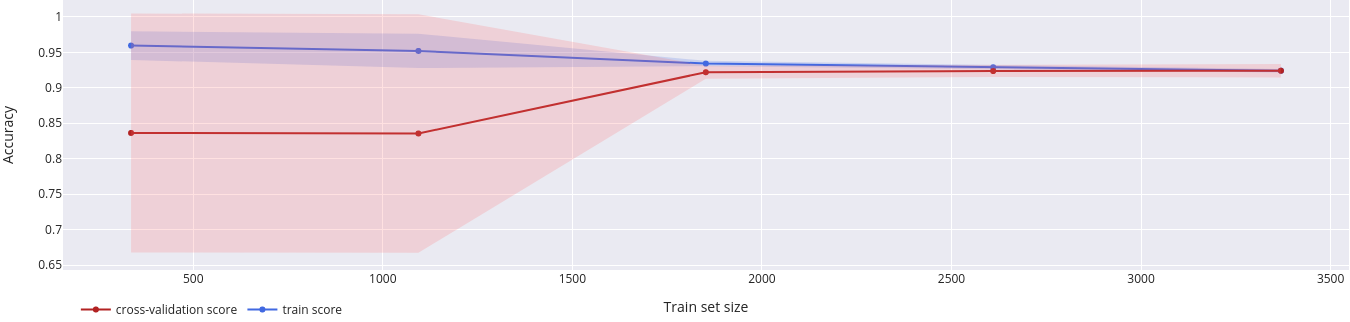
\includegraphics[width=\textwidth]{plots/classification/naive_bayes_learning_curve.png}
    	\label{fig:random_forest_learning_curve}
    	\subcaption{Naive Bayes}
	\end{minipage}
	\captionof{figure}{Learning curve for different algorithms.}
\end{figure}


\begin{table}[h]
\centering
\begin{tabular}{l|llll|llll|}
\cline{2-9}
                                              & \multicolumn{4}{c|}{\textbf{\begin{tabular}[c]{@{}c@{}}Validation\\ (SMOTE)\end{tabular}}}                                             & \multicolumn{4}{c|}{\textbf{\begin{tabular}[c]{@{}c@{}}Validation\\ (Unbalanced)\end{tabular}}}                                        \\ \hline
\multicolumn{1}{|c|}{\textbf{Algorithm}}      & \multicolumn{1}{c|}{\textbf{A}} & \multicolumn{1}{c|}{\textbf{F1}} & \multicolumn{1}{c|}{\textbf{P}} & \multicolumn{1}{c|}{\textbf{R}} & \multicolumn{1}{c|}{\textbf{A}} & \multicolumn{1}{c|}{\textbf{F1}} & \multicolumn{1}{c|}{\textbf{P}} & \multicolumn{1}{c|}{\textbf{R}} \\ \hline
\multicolumn{1}{|l|}{\textbf{Decision Tree}}  & \multicolumn{1}{l|}{.96}        & \multicolumn{1}{l|}{.96}         & \multicolumn{1}{l|}{.96}        & .96                             & \multicolumn{1}{l|}{.95}        & \multicolumn{1}{l|}{.89}         & \multicolumn{1}{l|}{.91}        & .87                             \\ \hline
\multicolumn{1}{|l|}{\textbf{Rule Based}}     & \multicolumn{1}{l|}{.92}        & \multicolumn{1}{l|}{.92}         & \multicolumn{1}{l|}{.93}        & .91                             & \multicolumn{1}{l|}{.95}        & \multicolumn{1}{l|}{.88}         & \multicolumn{1}{l|}{.86}        & .90                             \\ \hline
\multicolumn{1}{|l|}{\textbf{Random Forest}}  & \multicolumn{1}{l|}{.96}        & \multicolumn{1}{l|}{.96}         & \multicolumn{1}{l|}{.95}        & .98                             & \multicolumn{1}{l|}{.96}        & \multicolumn{1}{l|}{.91}         & \multicolumn{1}{l|}{.90}        & .90                             \\ \hline
\multicolumn{1}{|l|}{\textbf{AdaBoost}}       & \multicolumn{1}{l|}{.96}        & \multicolumn{1}{l|}{.96}         & \multicolumn{1}{l|}{.94}        & .97                             & \multicolumn{1}{l|}{.95}        & \multicolumn{1}{l|}{.89}         & \multicolumn{1}{l|}{.89}        & .89                             \\ \hline
\multicolumn{1}{|l|}{\textbf{KNN}}            & \multicolumn{1}{l|}{.96}        & \multicolumn{1}{l|}{.96}         & \multicolumn{1}{l|}{.94}        & .99                             & \multicolumn{1}{l|}{.95}        & \multicolumn{1}{l|}{.90}         & \multicolumn{1}{l|}{.88}        & .91                             \\ \hline
\multicolumn{1}{|l|}{\textbf{Naive Bayes}}    & \multicolumn{1}{l|}{.92}        & \multicolumn{1}{l|}{.92}         & \multicolumn{1}{l|}{.93}        & .91                             & \multicolumn{1}{l|}{.93}        & \multicolumn{1}{l|}{.85}         & \multicolumn{1}{l|}{.80}        & .91                             \\ \hline
\multicolumn{1}{|l|}{\textbf{SVM}}            & \multicolumn{1}{l|}{.98}        & \multicolumn{1}{l|}{.98}         & \multicolumn{1}{l|}{.97}        & .98                             & \multicolumn{1}{l|}{.96}        & \multicolumn{1}{l|}{.91}         & \multicolumn{1}{l|}{.92}        & .90                             \\ \hline
\multicolumn{1}{|l|}{\textbf{Neural Network}} & \multicolumn{1}{l|}{.97}        & \multicolumn{1}{l|}{.97}         & \multicolumn{1}{l|}{.96}        & .98                             & \multicolumn{1}{l|}{.96}        & \multicolumn{1}{l|}{.91}         & \multicolumn{1}{l|}{.92}        & .89                             \\ \hline
\end{tabular}
\caption{Validation metrics for all the models on the normal dataset and on the SMOTE dataset.}
\label{tab:metrics-validation}
\end{table}

The best parameters obtained through the grid search can be found for each classifier in the attached notebook.

\subsubsection{Decision Tree interpretability}
\begin{figure}[h!]
	\centering
	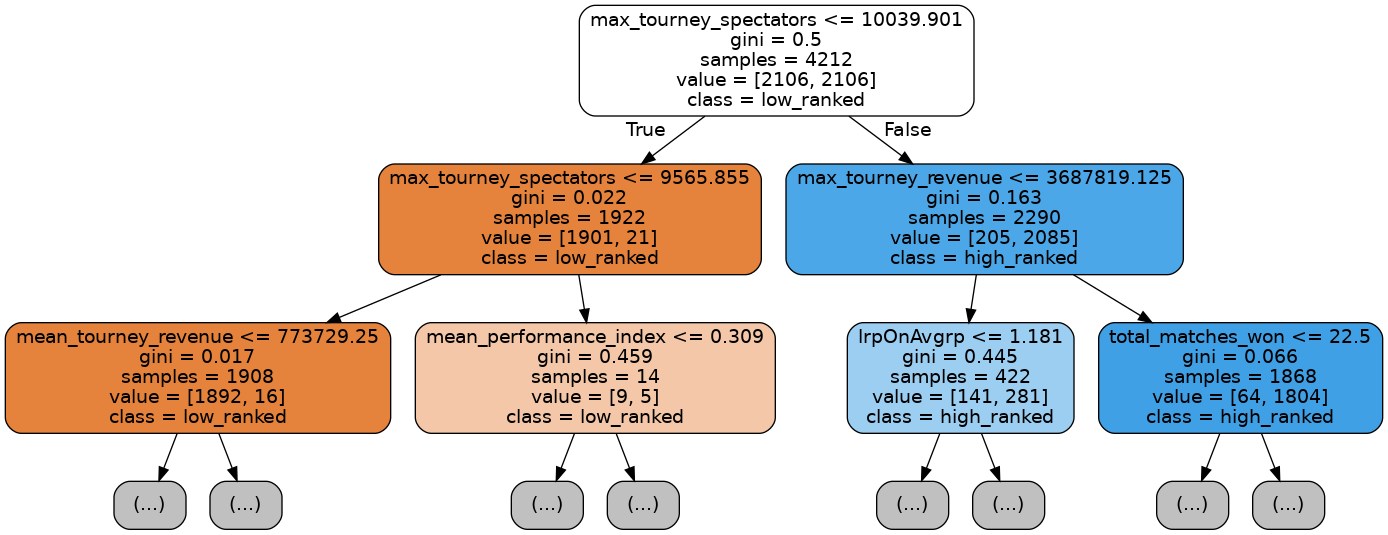
\includegraphics[width=\textwidth]{plots/classification/decision_tree_plot.png}
	\captionof{figure}{First 3 levels of the Decision Tree.}
	\label{fig:decision_tree_plot}
\end{figure}
The decision tree performed very well. The best model in terms of accuracy has a \verb|max_depth| of 12, but we preferred to choose a model with a depth of 8 in order to have a better interpretability. With this move, the accuracy on validation dropped just a little (from 0.9648 to 0.9634). It seemed to be a good strategy keeping in mind Occam's razor and also because as can be seen in the validation curve in Figure \ref{fig:decision_tree_curve}, the standard deviation when the depth is 8 is narrower than its counterpart with 14, where there seems to be a slight overfitting. This ensures that is statistically more significant.

\begin{figure}[h!]
	\centering
	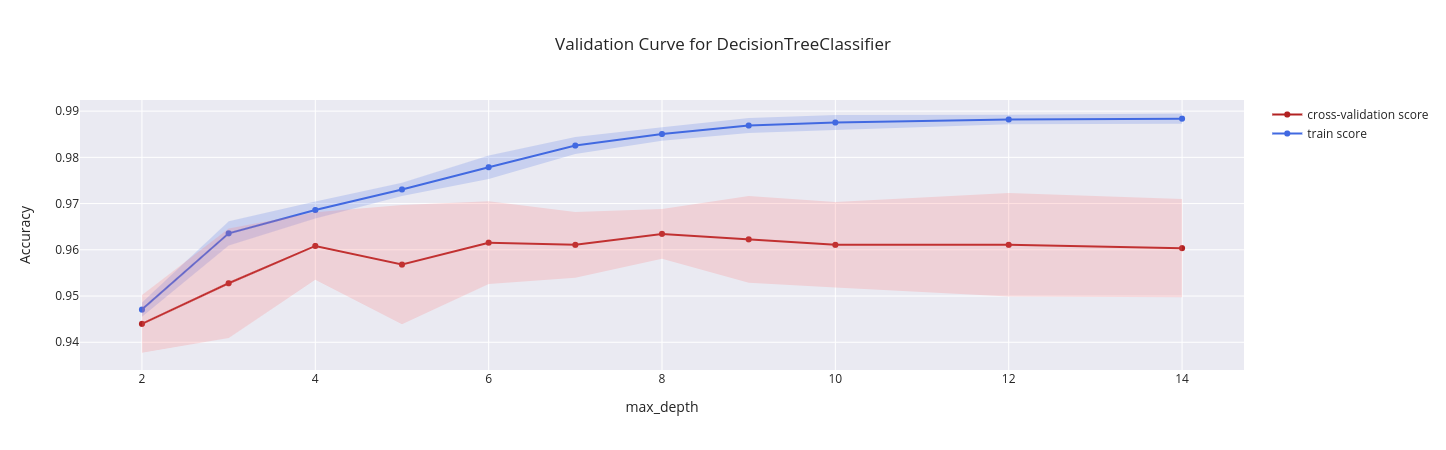
\includegraphics[width=\textwidth]{plots/classification/decision_tree_validation_curve.png}
	\captionof{figure}{Learning curve decision tree}
	\label{fig:decision_tree_curve}
\end{figure}


As we can see in Figure \ref{fig:decision_tree_plot}, the first and most significant split is made on \textit{max\_tourney\_spectators}. An interesting thing to note is that the left node of the first level has a very low impurity with respect to the right one. This happens because the ones who have never played in a big tourney (with a large amount of spectators), are basically low-ranked, while a discrete amount of low-ranked players could play in important tourneys from time to time. The following splits are made on other features describing the importance of the tourneys in which players have played and their performance.

Let's open a digression for the rule based classifiers, more specifically we used \textbf{RIPPER} which in general should have similar performance to a decision tree implemented with the CART algorithm. Even this classifier mainly discriminated the players based on the above-mentioned features, such as \textit{max\_tourney\_spectators} and \textit{max\_tourney\_revenue}. Obviously, the importance of some minor features differ, but this is also true for the decision tree when initializing with different random seeds.\\

\subsection{Comparison}
\begin{figure}[h]
	\centering
	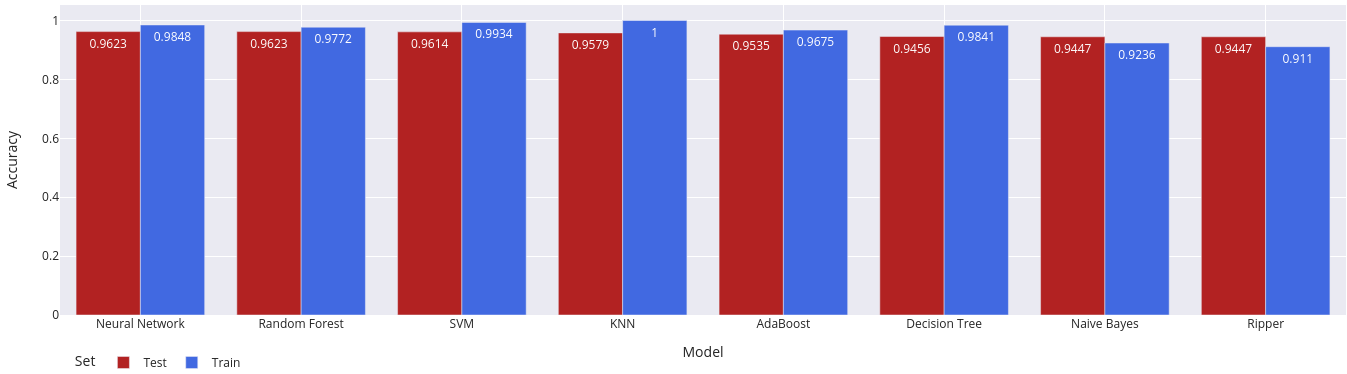
\includegraphics[width=\textwidth]{plots/classification/accuracy.png}
	\captionof{figure}{Accuracy on test set (red) and training set (blue).}
	\label{fig:accuracy}
\end{figure}
After carrying out the analysis and identifying the best models through cross validation, we obtained the following results shown in Figure \ref{fig:test_metrics} (the precision and the recall reported are about the \texit{high\_ranked} class, which is also the one with the smallest number of instances). Due to the fact that the test dataset is unbalanced, a ROC curve could provide optimistic results. Accuracy may also be subject to over-optimistic bias, so we can analyse the best performance of the models using the F1 metric. So it is easy to see that the best models are, Random Forest (91.38\%), Neural Network (91.06\%), and SVM (90.79\%). It is also interesting to note that the worst models that are Decision Tree and Rule Based are also the ones that have the best explainability.

\begin{figure}[h]
	\centering
	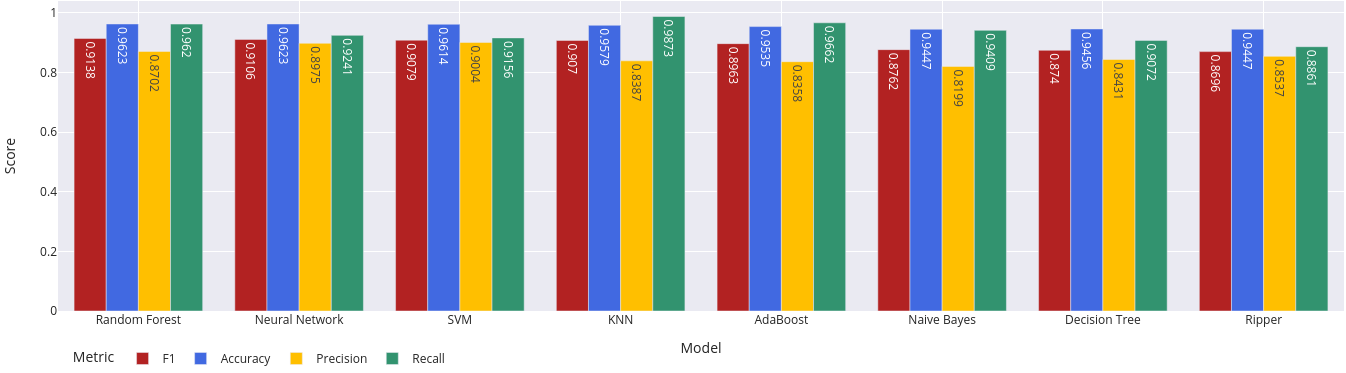
\includegraphics[width=\textwidth]{plots/classification/test_metrics.png}
	\captionof{figure}{Test metrics}
	\label{fig:test_metrics}
\end{figure}

\subsubsection{Digression on K-means}
In addition to the above, we would like to point out that our clustering analysis (Sec. \ref{sec:clustering}) had already identified a partitioning between strong and weak players. A k-means with a k=2 in fact identifies precisely the strong and weak players (Fig. \ref{fig:k_means_comparison} (b)), and the distribution seems to be Pareto. This is in line with what was said during the decision for the label extraction.

We can in fact appreciate and visualize through a PCA (Fig. \ref{fig:k_means_comparison} (a)) the classification carried out by one of the best algorithms, namely the Random Forest, which by looking at the same visualization vaguely reminds us the distinction performed by the clustering algorithm.

\begin{figure}[h]
	\centering
	\begin{minipage}{.48\textwidth}
	    \centering
    	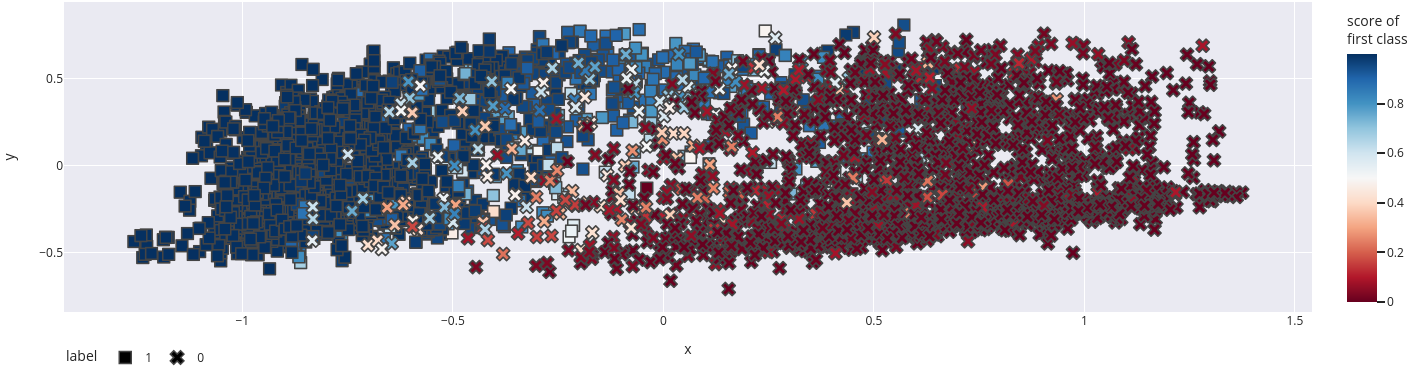
\includegraphics[width=\textwidth]{plots/classification/random_forest_pca.png}
    	\label{fig:random_forest_pca}
    	\subcaption{Random Forest PCA visualization}
	\end{minipage}
	\begin{minipage}{.48\textwidth}
	    \centering
		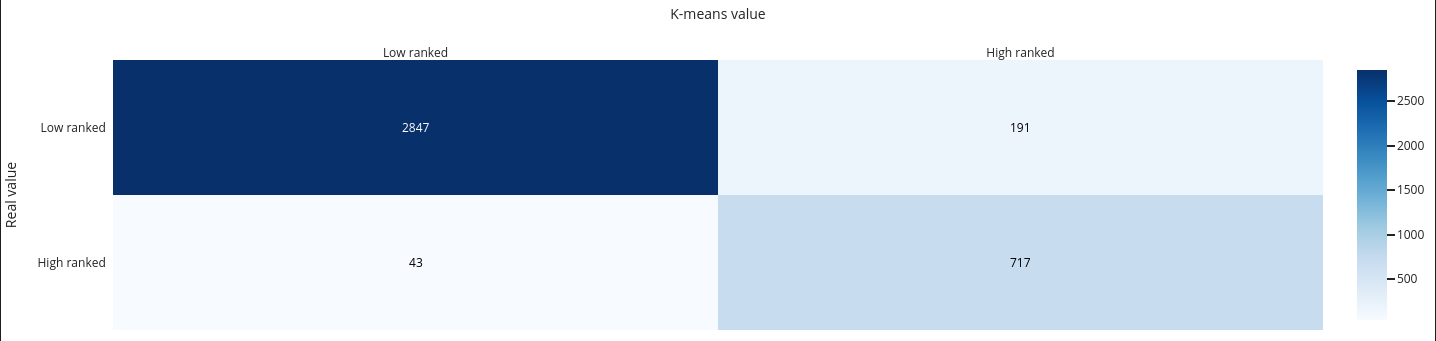
\includegraphics[width=\textwidth]{plots/classification/confusion_matrix_kmeans.png}
    	\label{fig:k_means_classification}
    	\subcaption{K-means with respect to the label}
	\end{minipage}
	\captionof{figure}{Comparison with clustering.}
	\label{fig:k_means_comparison}
\end{figure}